\documentclass[oneside,openany,headings=optiontotoc,11pt,numbers=noenddot]{scrreprt}

\usepackage[a4paper]{geometry}
\usepackage[utf8]{inputenc}
\usepackage[T1]{fontenc}
\usepackage{lmodern}
\usepackage[ngerman]{babel}
\usepackage{ngerman}

\usepackage[onehalfspacing]{setspace}

\usepackage{fancyhdr}
\usepackage{fancybox}

\usepackage{rotating}
\usepackage{varwidth}

%Struktogramme
\usepackage[german,curves]{struktex}

\usepackage{pdflscape}
\usepackage{changepage}
\usepackage{graphicx}
\usepackage[bottom]{footmisc}
\usepackage{transparent}
\usepackage{graphbox}
\graphicspath{
	{Pics/PDFs/}
	{Pics/JPGs/}
	{Pics/PNGs/}
}
\usepackage{caption}
\usepackage{wrapfig}
\usepackage{marginnote}
\usepackage{tabularx}
\usepackage{dashrule}
\usepackage{soulutf8}
\usepackage{hhline}
%arydshln suppresses vertical lines in table
%\usepackage{arydshln}
\usepackage{multirow}
\usepackage{enumerate}
\usepackage[hidelinks]{hyperref}
\usepackage{listings}

\usepackage[table]{xcolor}
\usepackage{array}
\usepackage{enumitem,amssymb,amsmath}
\usepackage{interval}
\usepackage{cancel}
\usepackage{stmaryrd}
\usepackage{wasysym}
\usepackage{polynom}
\usepackage{diagbox}
\usepackage{dashrule}
\usepackage{framed}
\usepackage{mdframed}
\usepackage{karnaugh-map}
\usepackage{pdfpages}

\usepackage{blindtext}

\usepackage{eso-pic}

\usepackage{amssymb}
\usepackage{eurosym}

\usepackage[pages=some]{background}
\pagestyle{headings}
\renewcommand{\headrulewidth}{0.2pt}
\renewcommand{\footrulewidth}{0.2pt}
\newcommand*{\underdownarrow}[2]{\ensuremath{\underset{\overset{\Big\downarrow}{#2}}{#1}}}
\setlength{\fboxsep}{5pt}
\newcommand{\explainBelow}[3]{\underbrace{#1}_{\parbox{\widthof{#3}}{\footnotesize\raggedright #2}}}
\newcommand{\explainAbove}[3]{\overbrace{#1}^{\parbox{\widthof{#3}}{\footnotesize\raggedright #2}}}
\newcommand\footnoteref[1]{\protected@xdef\@thefnmark{\ref{#1}}\@footnotemark}


% Codestyle defined
\definecolor{codegreen}{rgb}{0,0.6,0}
\definecolor{codegray}{rgb}{0.5,0.5,0.5}
\definecolor{codepurple}{rgb}{0.58,0,0.82}
\definecolor{backcolour}{rgb}{0.95,0.95,0.92}
\definecolor{deepgreen}{rgb}{0,0.5,0}
\definecolor{darkblue}{rgb}{0,0,0.65}
\definecolor{mauve}{rgb}{0.40, 0.19,0.28}
\colorlet{exceptioncolour}{yellow!50!red}
\colorlet{commandcolour}{blue!60!black}
\colorlet{numpycolour}{blue!60!green}
\colorlet{specmethodcolour}{violet}

%Neue Spaltendefinition
\newcolumntype{L}[1]{>{\raggedright\let\newline\\\arraybackslash\hspace{0pt}}m{#1}}
\newcolumntype{M}{>{\centering\arraybackslash}X}
\newcommand{\cmnt}[1]{\ignorespaces}
%Textausrichtung ändern
\newcommand\tabrotate[1]{\rotatebox{90}{\raggedright#1\hspace{\tabcolsep}}}

%Intervall-Konfig
\intervalconfig {
	soft open fences
}

%Bash
\lstdefinestyle{BashInputStyle}{
	language=bash,
	basicstyle=\small\sffamily,
	backgroundcolor=\color{backcolour},
	columns=fullflexible,
	backgroundcolor=\color{backcolour},
	breaklines=true,
}
%Java
\lstdefinestyle{JavaInputStyle}{
	language=Java,
	backgroundcolor=\color{backcolour},
	aboveskip=1mm,
	belowskip=1mm,
	showstringspaces=false,
	columns=flexible,
	basicstyle={\footnotesize\ttfamily},
	numberstyle={\tiny},
	numbers=none,
	keywordstyle=\color{purple},,
	commentstyle=\color{deepgreen},
	stringstyle=\color{blue},
	emph={out},
	emphstyle=\color{darkblue},
	emph={[2]rand},
	emphstyle=[2]\color{specmethodcolour},
	breaklines=true,
	breakatwhitespace=true,
	tabsize=2,
}
%Python
\lstdefinestyle{PythonInputStyle}{
	language=Python,
	alsoletter={1234567890},
	aboveskip=1ex,
	basicstyle=\footnotesize,
	breaklines=true,
	breakatwhitespace= true,
	backgroundcolor=\color{backcolour},
	commentstyle=\color{red},
	otherkeywords={\ , \}, \{, \&,\|},
	emph={and,break,class,continue,def,yield,del,elif,else,%
		except,exec,finally,for,from,global,if,import,in,%
		lambda,not,or,pass,print,raise,return,try,while,assert},
	emphstyle=\color{exceptioncolour},
	emph={[2]True,False,None,min},
	emphstyle=[2]\color{specmethodcolour},
	emph={[3]object,type,isinstance,copy,deepcopy,zip,enumerate,reversed,list,len,dict,tuple,xrange,append,execfile,real,imag,reduce,str,repr},
	emphstyle=[3]\color{commandcolour},
	emph={[4]ode, fsolve, sqrt, exp, sin, cos, arccos, pi,  array, norm, solve, dot, arange, , isscalar, max, sum, flatten, shape, reshape, find, any, all, abs, plot, linspace, legend, quad, polyval,polyfit, hstack, concatenate,vstack,column_stack,empty,zeros,ones,rand,vander,grid,pcolor,eig,eigs,eigvals,svd,qr,tan,det,logspace,roll,mean,cumsum,cumprod,diff,vectorize,lstsq,cla,eye,xlabel,ylabel,squeeze},
	emphstyle=[4]\color{numpycolour},
	emph={[5]__init__,__add__,__mul__,__div__,__sub__,__call__,__getitem__,__setitem__,__eq__,__ne__,__nonzero__,__rmul__,__radd__,__repr__,__str__,__get__,__truediv__,__pow__,__name__,__future__,__all__},
	emphstyle=[5]\color{specmethodcolour},
	emph={[6]assert,range,yield},
	emphstyle=[6]\color{specmethodcolour}\bfseries,
	emph={[7]Exception,NameError,IndexError,SyntaxError,TypeError,ValueError,OverflowError,ZeroDivisionError,KeyboardInterrupt},
	emphstyle=[7]\color{specmethodcolour}\bfseries,
	emph={[8]taster,send,sendMail,capture,check,noMsg,go,move,switch,humTem,ventilate,buzz},
	emphstyle=[8]\color{blue},
	keywordstyle=\color{blue}\bfseries,
	rulecolor=\color{black!40},
	showstringspaces=false,
	stringstyle=\color{deepgreen}
}

\lstset{literate=%
	{Ö}{{\"O}}1
	{Ä}{{\"A}}1
	{Ü}{{\"U}}1
	{ß}{{\ss}}1
	{ü}{{\"u}}1
	{ä}{{\"a}}1
	{ö}{{\"o}}1
}

% Neue Klassenarbeits-Umgebung
\newenvironment{worksheet}[3]
% Begin-Bereich
{
	\newpage
	\sffamily
	\setcounter{page}{1}
	\ClearShipoutPicture
	\AddToShipoutPicture{
		\put(55,761){{
				\mbox{\parbox{385\unitlength}{\tiny \color{codegray}BBS I Mainz, #1 \newline #2
						\newline #3
					}
				}
			}
		}
		\put(455,761){{
				\mbox{\hspace{0.3cm}
\includegraphics[width=0.2\textwidth]{../../logo.pdf}}
			}
		}
	}
}
% End-Bereich
{
	\clearpage
	\ClearShipoutPicture
}

\geometry{left=2.50cm,right=2.50cm,top=2.00cm,bottom=1.00cm,includeheadfoot}

\begin{document}
	\begin{worksheet}{HBF IT 17A}{Grundstufe}{Vorbereitung Klassenarbeit - Lösung}
		\begin{framed}
			\noindent\normalsize
			Beschreiben Sie das \textbf{Verhalten} der folgenden Funktionen \textbf{für große bzw. kleine x-Werte}.
			\begin{framed}
				Beachten Sie die Schreibweise \(f(x) \xrightarrow{x \rightarrow -\infty}\) / \(f(x) \xrightarrow{x \rightarrow \infty}\)
			\end{framed}
			\begin{itemize}
				\item[(a)] \(f(x) = 3x^6 -18x^4 +27x^2\)\\
				betrachte \(3x^6\)\\
				\(a_n\) positiv und \(n\) gerade:\\
				\(f(x) \xrightarrow{x \rightarrow -\infty} \infty\)\\
				\(f(x) \xrightarrow{x \rightarrow \infty} \infty\)
				\item[(b)] \(f(x) = -0.9x^7+10x^3\)\\
				betrachte \(-0.9x^7\)\\
				\(a_n\) negativ und \(n\) ungerade:\\
				\(f(x) \xrightarrow{x \rightarrow -\infty} \infty\)\\
				\(f(x) \xrightarrow{x \rightarrow \infty} -\infty\)
				\item[(c)] \(f(x) = -5x^4 +20x^3 -12x^2 +8\)\\
				betrachte \(-5x^4\)\\
				\(a_n\) negativ und \(n\) gerade:\\
				\(f(x) \xrightarrow{x \rightarrow -\infty} \infty\)\\
				\(f(x) \xrightarrow{x \rightarrow \infty} -\infty\)
				\item[(d)] \(f(x) = 0.8x^5-5x^3-x\)\\
				betrachte \(0.8x^5\)\\
				\(a_n\) positiv und \(n\) ungerade:\\
				\(f(x) \xrightarrow{x \rightarrow -\infty} -\infty\)\\
				\(f(x) \xrightarrow{x \rightarrow \infty} \infty\)
			\end{itemize}
			\hdashrule[0.5ex][x]{\textwidth}{0.1mm}{8mm 2pt}\\
			\newpage
			Ordnen Sie die Graphen der Ableitungsfunktionen \(f'(x)\) den richtigen Ausgangsgraphen für \(f(x)\) zu.\\
			Begründen Sie ihre Entscheidung in Stichpunkten.\\
			\begin{tabularx}{\textwidth}{|cX|cX|cX|}
				\hline
				\multicolumn{6}{|l|}{Ausgangsgraph von \(f(x)\)}\\
				\hline
				(a) & & (b) & & (c) &\\
				& 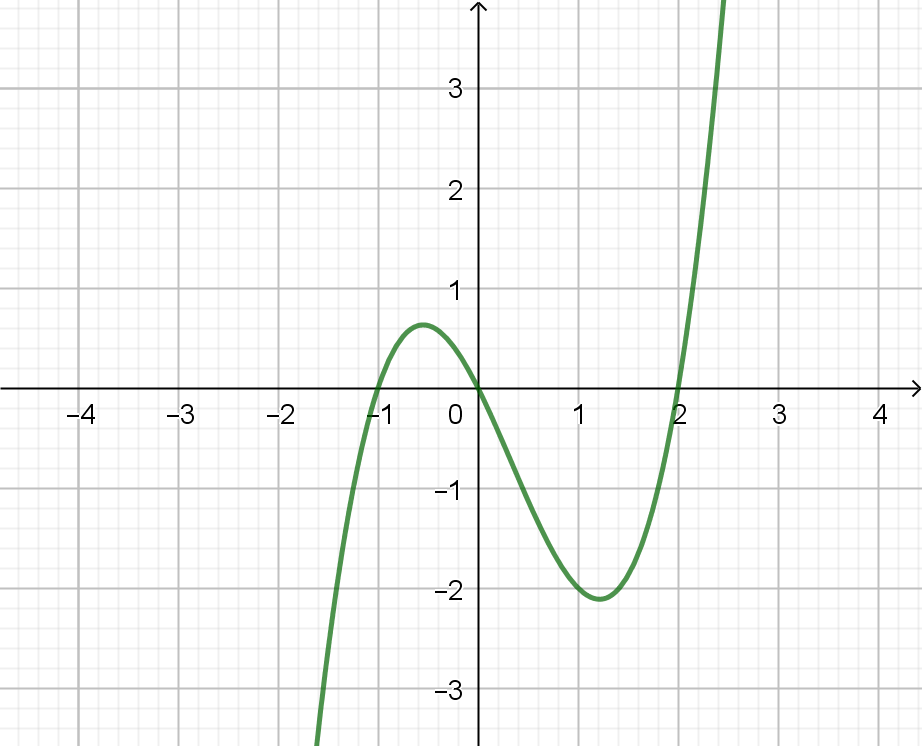
\includegraphics[scale=0.2]{Bilder/fue.png} & & 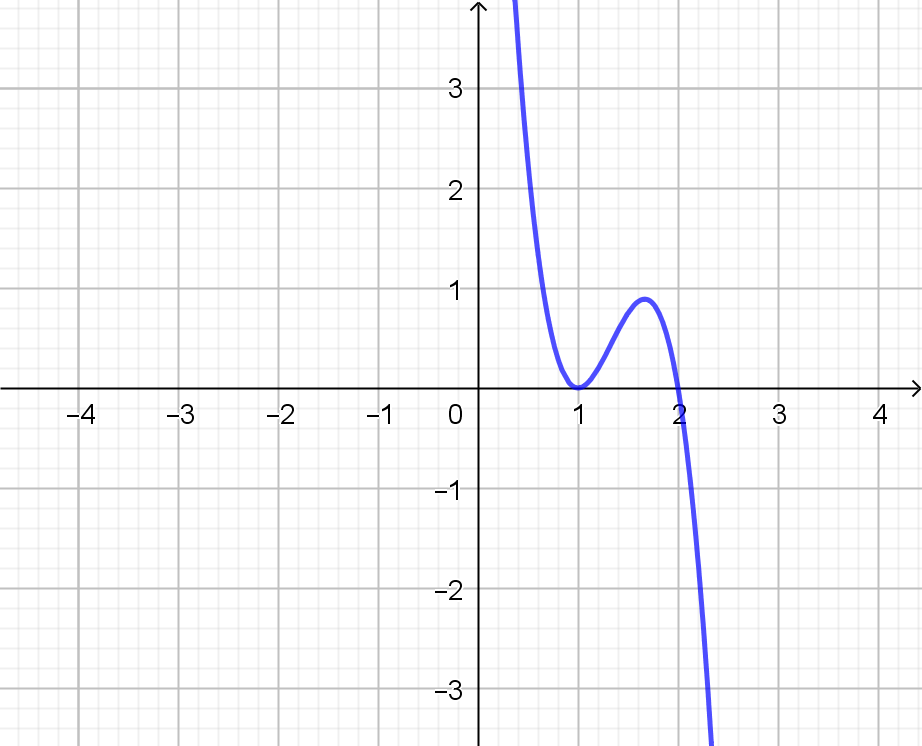
\includegraphics[scale=0.2]{Bilder/gue.png} & & 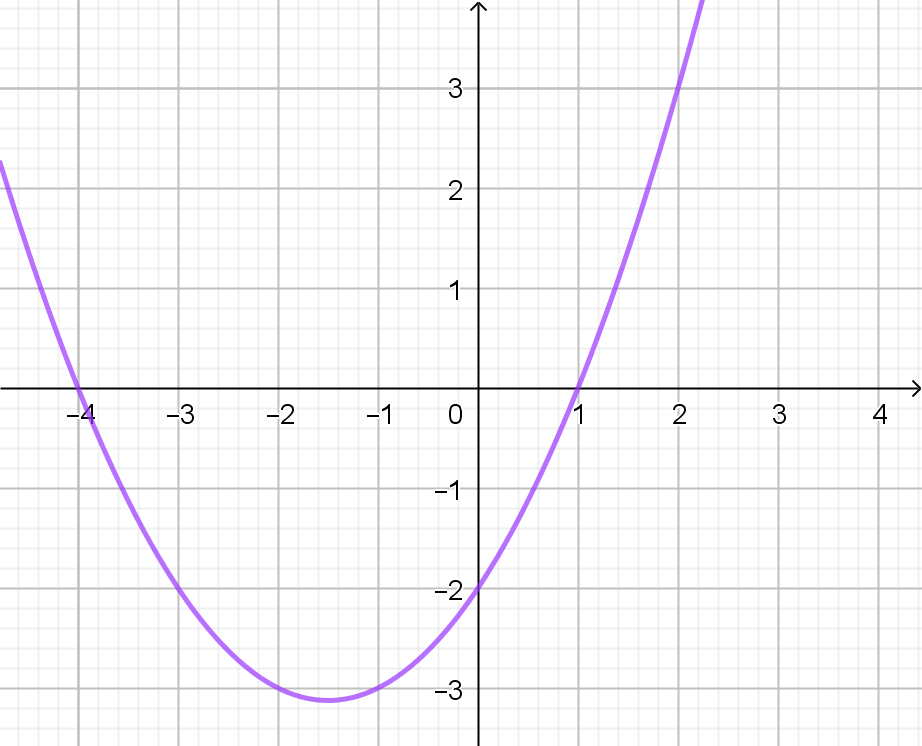
\includegraphics[scale=0.2]{Bilder/hue.png}\\
				\hline
				\multicolumn{6}{|l|}{Graph der Ableitungsfunktion \(f'(x)\)}\\
				\hline
				(1) & & (2) & & (3) &\\
				& 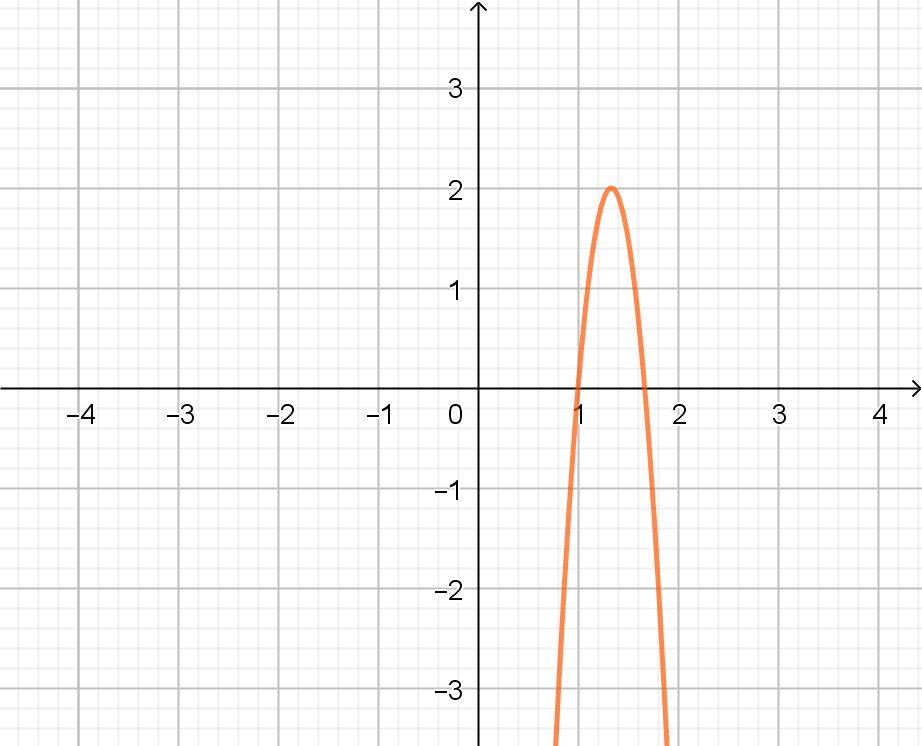
\includegraphics[scale=0.2]{Bilder/g'ue.png} & & 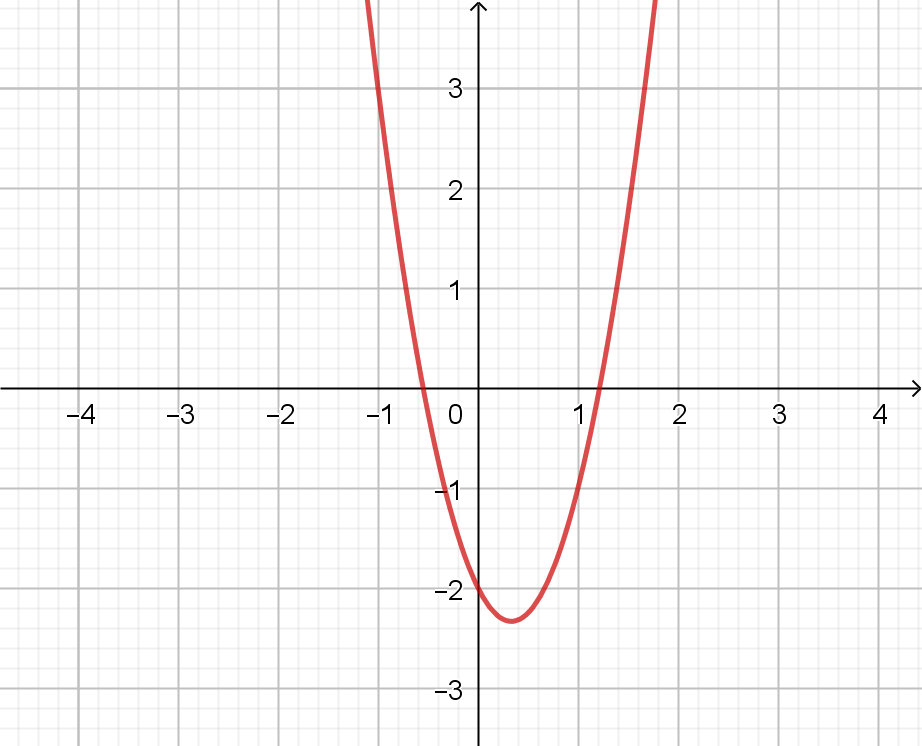
\includegraphics[scale=0.2]{Bilder/f'ue.png} & & 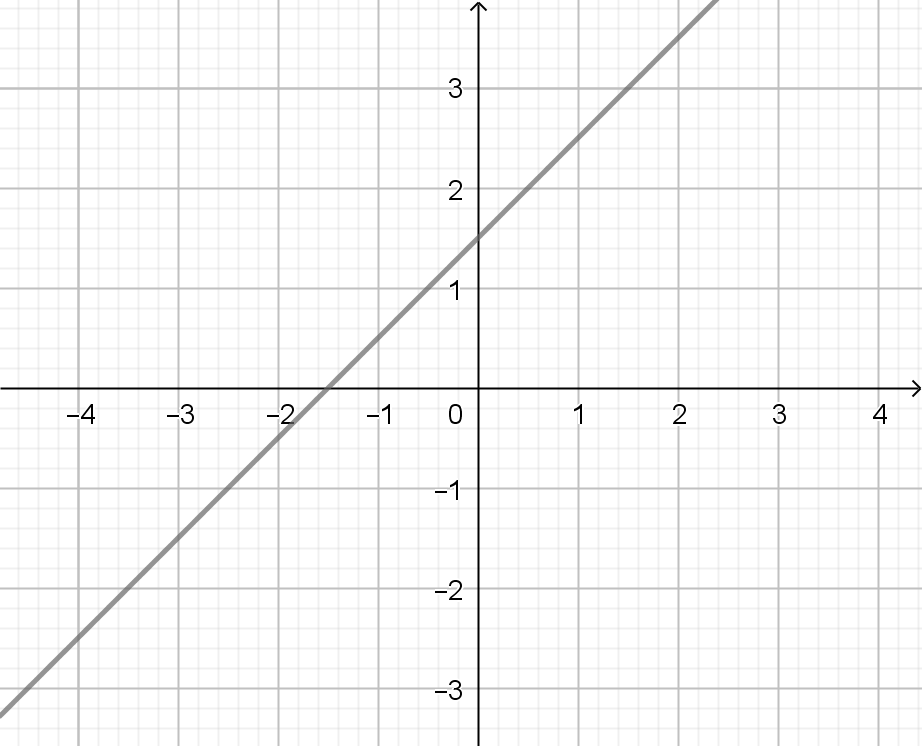
\includegraphics[scale=0.2]{Bilder/h'ue.png}\\
				\hline
			\end{tabularx}\\
			\par\bigskip\noindent
			Ausgangsgraph (a) gehört zum Ableitungsgraph (2)
			\begin{itemize}
				\item Ausgangsgraph ist eine Funktion 3. Grades und hat Extrempunkte bei \(x=0.5\) und ca. \(x=1.2\). Der Ableitungsgraph (b) ist 2. Grades und hat Nullstellen bei \(x=0.5\) und \(x=1.2\) (Wir wissen, \(f(x) \) ist Extrempunkt wenn \(f'(x)=0\))\\
				Die Steigung vor dem ersten Extrempunkt \(x<0.5\) ist positiv (Ableitungsgraph oberhalb der x-Achse), für \(0.5 < x < 1.2\) ist die Steigung negativ (Ableitungsgraph unterhalb der x-Achse) und die Steigung nach dem zweiten Extrempunkt \(1.2<x\) ist wieder positiv (Ableitungsgraph oberhalb der x-Achse).
			\end{itemize}
			Ausgangsgraph (b) gehört zu Ableitungsgraph (1)
			\begin{itemize}
 				\item Ausgangsgraph ist eine Funktion 3. Grades und hat Extrempunkte bei ca. \(x=1\) und ca. \(x=1.75\). Der Ableitungsgraph (b) ist 2. Grades und hat Nullstellen bei ungefähr \(x=1\) und \(x=1.75\) (Wir wissen, \(f(x) \) ist Extrempunkt wenn \(f'(x)=0\))\\
 				Die Steigung vor dem ersten Extrempunkt \(x<1\) ist negativ (Ableitungsgraph unterhalb der x-Achse), für \(1 < x < 1.75\) ist die Steigung positiv (Ableitungsgraph oberhalb der x-Achse) und die Steigung nach dem zweiten Extrempunkt \(1.75<x\) ist wieder negativ (Ableitungsgraph unterhalb der x-Achse).
			\end{itemize}
			Ausgangsgraph (c) gehört zu Ableitungsgraph (3)
			\begin{itemize}
				\item Ausgangsgraph ist eine Funktion 2. Grades und hat einen Extrempunkt bei ca. \(x=-1.5\). Der Ableitungsgraph (b) ist linear, also 1. Grades und hat genau eine Nullstellen bei ungefähr \(x=-1.5\) (Wir wissen, \(f(x) \) ist Extrempunkt wenn \(f'(x)=0\))\\
				Die Steigung vor dem Extrempunkt \(x<-1.5\) ist negativ (Ableitungsgraph unterhalb der x-Achse), nach dem Extrempunkt \(-1.5<x\) ist positiv (Ableitungsgraph oberhalb der x-Achse).
			\end{itemize}
			\hdashrule[0.5ex][x]{\textwidth}{0.1mm}{8mm 2pt}\\
			\textbf{Skizzieren} Sie den Graphen der Ableitungsfunktion zu gegebenem Funktionsgraphen.\\
			Tun Sie dies im gleichen Koordinatensystem.\\
			\textbf{Beschreiben} Sie ihr Vorgehen in Stichpunkten.\\
			\begin{center}
				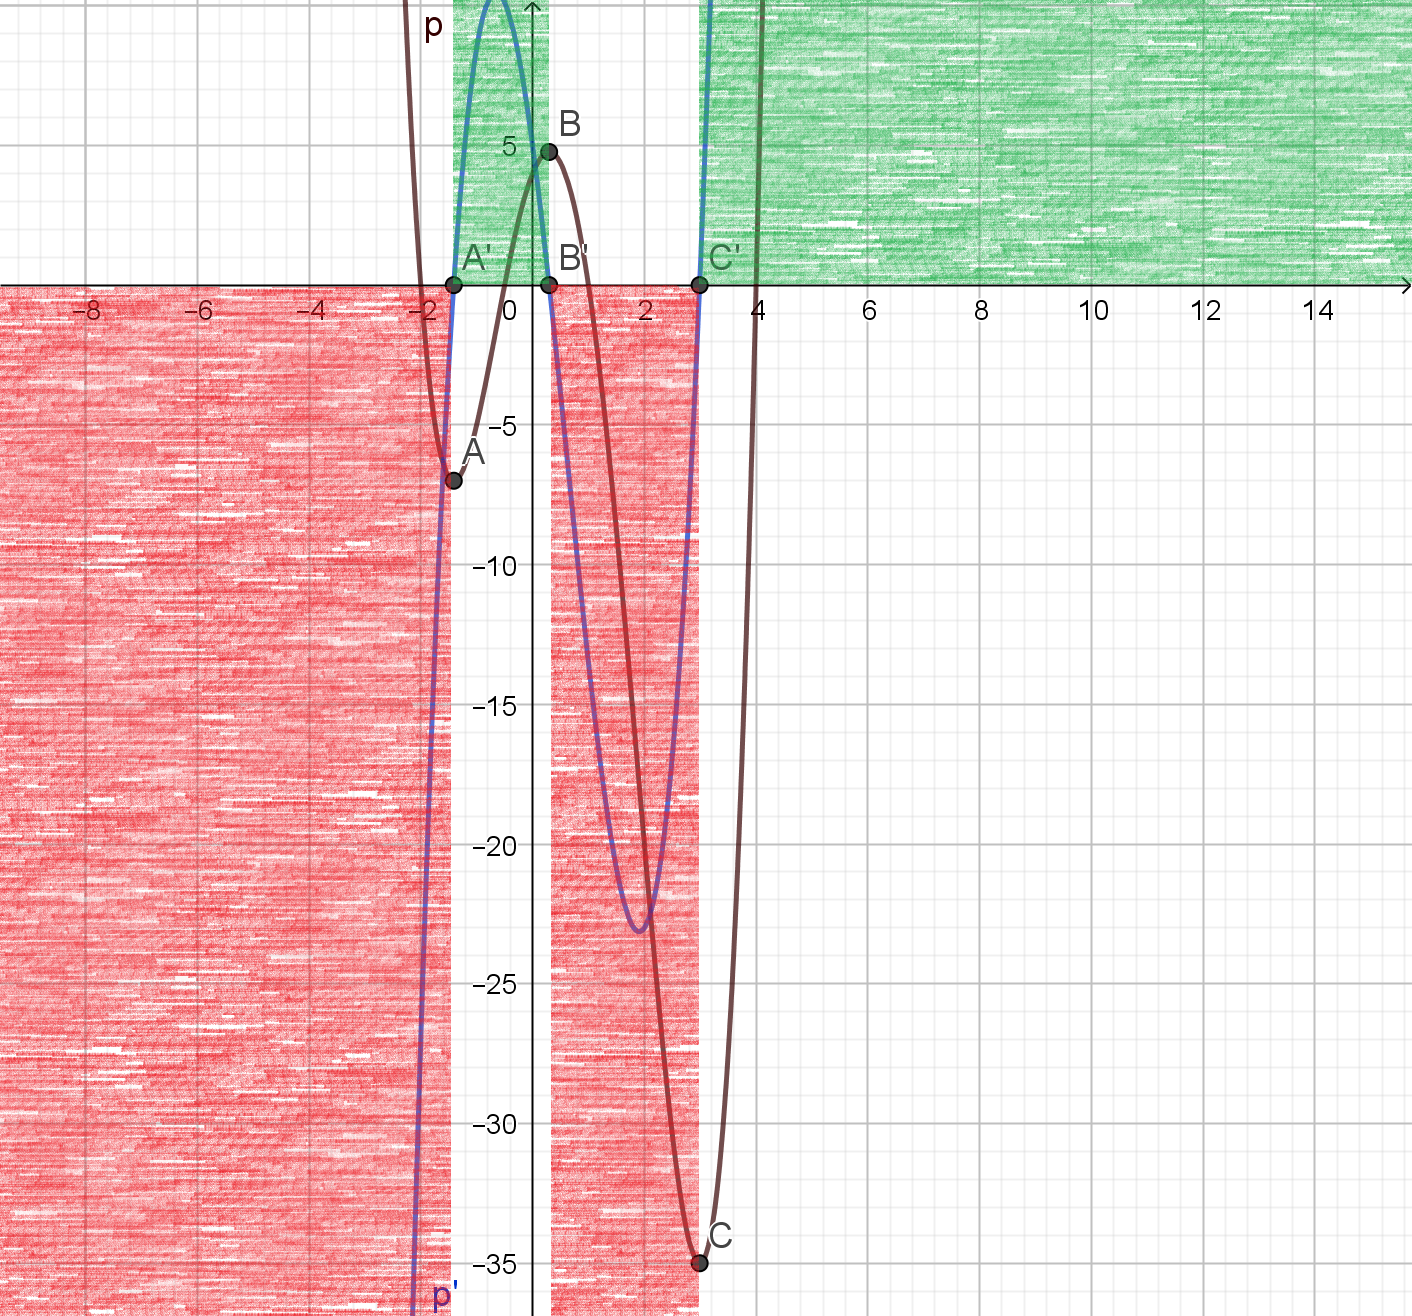
\includegraphics[scale=0.6]{Bilder/pp'ue.png}
			\end{center}
			\hdashrule[0.5ex][x]{\textwidth}{0.1mm}{8mm 2pt}
			\newpage
			\noindent
			Bestimmen Sie rechnerisch die \textbf{Nullstellen} der Funktionen:\\
			(a) \(f(x) = x^3 -4.5x^2+5x\)\\
			\par\bigskip\noindent
			\begin{tabularx}{\textwidth}{XXX}
				\(0 = x^3 -4.5x^2 +5x\)  & \multicolumn{2}{l}{| \(x\) in jedem Term vorhanden \(\Rightarrow\) \textbf{x ausklammern}.}\\
				\(0 = \underbrace{x}_{=0 \text{ oder }}*\underbrace{(x^2 -4.5x +5)}_{=0}\) & \multicolumn{2}{l}{| Ein Produkt \(a*b = 0\), wenn ein Faktor \(a= 0\) oder \(b=0\).}\\
				\hline\\
				\multicolumn{1}{l|}{\(x = 0\)} & \(x^2\underbrace{-4.5}_{p} x+\underbrace{5}_{q}\) & | pq-Formel\\
				\multicolumn{1}{l|}{}& \(x_{1,2} = -\frac{-4.5}{2}\pm\sqrt{(\frac{-4.5}{2})^2 -5}\)\\
				\multicolumn{1}{l|}{}& \(x_1 = \frac{4.5}{2}-\sqrt{(\frac{-4.5}{2})^2 -5}\) & \(x_2 = \frac{4.5}{2}+\sqrt{(\frac{-4.5}{2})^2 -5}\)\\
				\multicolumn{1}{l|}{} & \(x_1 = 2\) & \(x_2 = 2.5\)
			\end{tabularx}
			\par\bigskip\noindent
			(b) \(f(x) = x^2 -1\)\\
			\par\bigskip\noindent
			\begin{tabularx}{\textwidth}{XXX}
				\(0 = x^2 - 1\)  & \multicolumn{2}{l}{| \(x\) nur in einem Term vorhanden. Nach \(x\) umformen.}\\
				\(1 = x^2\) & | \(\sqrt{}\)\\
				\(x_1 = +\sqrt{1}\) & \(x_2 = -\sqrt{1}\)\\
			\end{tabularx}
			\par\bigskip\noindent
			\hdashrule[0.5ex][x]{\textwidth}{0.1mm}{8mm 2pt}\\
			Ermitteln Sie rechnerisch die \textbf{Extrempunkte} der Funktionen:\\
			\par\noindent
			(a) \(f(x) = \frac{1}{4}x^4 + \frac{7}{3}x^3 +x^2-40x\)\\
			Wir bestimmen zunächst die Ableitung. \small{\textit{Wir wissen, \(x\) ist ein Extrempunkt, wenn \(f'(x) = 0\).}}\\
			\normalsize
			\begin{tabularx}{\textwidth}{XXX}
				\(f'(x) = x^3 +7x^2+2x-40\) & | Um die Extremstellen zu berechnen, setzen wir \(f'(x) = 0\)\\
				\(0 = x^3 +7x^2+2x-40\) & | Haben wir eine Funktion 3. Grades, so versuchen wir eine Nullstelle zu raten. Meist \(-2; -1; 0; 1\) oder \(2\).\\
			\end{tabularx}
			In unserem Fall ist \(x=2\) eine Nullstelle. Wir führen also die Polynomdivision mit \(f'(x):(x-2)\) durch.\\
			\polyset{style=C, div=:,vars=x}
			\polylongdiv{x^3+7x^2+2x-40}{x-2}\\
			Unser Ergebnis \(x^2 +\underbrace{9}_{p}x +\underbrace{20}_{q}\) ist eine quadratische Funktion auf die wir die pq-Formel anwenden können.\\
			\begin{tabularx}{\textwidth}{X|X}
				\(x_1 = -\frac{9}{2} + \sqrt{(-\frac{9}{2})^2 -20}\) & \(x_2 = -\frac{9}{2} - \sqrt{(-\frac{9}{2})^2 -20}\)\\
				\(x_1 = -4\) & \(x_2 = -5\)
			\end{tabularx}
			Um die Extrempunkte zu berechnen, setzen wir die errechneten x-Werte in \(f(x)\) ein. So ergibt sich\\
			\begin{tabularx}{\textwidth}{XXX}
				\(\mathbf{f(-5)} = 89.58\) & \(\mathbf{f(-4)} = 90.67\) & \(\mathbf{f(0)}= -53.33\)\\
				(-5|89.58) & (-4|90.67) & (0|-53.33)
			\end{tabularx}\\
			\par\bigskip\noindent
			(b) \(f(x) = \frac{1}{3}x^3 +0,75x^2 -2,5x\)\\
			Wir bestimmen wieder die Ableitung. \small{\textit{Denn wir wissen, \(x\) ist ein Extrempunkt, wenn \(f'(x) = 0\).}}\\
			\normalsize
			\begin{tabularx}{\textwidth}{XX}
				\(f'(x) = x^2 +1.5x-2.5\) &| Um die Extremstellen zu berechnen, setzen wir \(f'(x) = 0\)\\
				\(0 = x^2 +\underbrace{1.5}_{p}x\underbrace{-2.5}_{q}\) & | Wir haben eine quadratische Funktion, also nutzen wir die pq-Formel.\\
				\multicolumn{1}{X|}{\(x_1 = -\frac{1.5}{2} + \sqrt{(-\frac{1.5}{2})^2 -(-2.5)}\)} & \multicolumn{1}{X}{\(x_2 = -\frac{1.5}{2} - \sqrt{(-\frac{1.5}{2})^2 - (-2.5)}\)}\\
				\multicolumn{1}{X|}{\(x_1 = -\frac{1.5}{2} + \sqrt{(-\frac{1.5}{2})^2 + 2.5}\)} & \multicolumn{1}{X}{\(x_2 = -\frac{1.5}{2} - \sqrt{(-\frac{1.5}{2})^2 + 2.5)}\)}\\
				\multicolumn{1}{X|}{\(x_1 = 1\)} & \multicolumn{1}{X}{\(x_2 = -2.5\)}\\
			\end{tabularx}
			Um die Extrempunkte zu berechnen, setzen wir die errechneten x-Werte in \(f(x)\) ein. So ergibt sich\\
			\begin{tabularx}{\textwidth}{XX}
				\(\mathbf{f(-2.5)} = 5.73\) & \(\mathbf{f(1)} = -1.42\)\\
				(-2.5|5.73) & (1|-1.42)
			\end{tabularx}\\
			\par\bigskip\noindent
			(c) \(f(x) = \frac{1}{2}x^2 -4x\)\\
			Wir bestimmen zunächst die Ableitung. \small{\textit{Denn wir wissen, \(x\) ist ein Extrempunkt, wenn \(f'(x) = 0\).}}\\
			\normalsize
			\begin{tabularx}{\textwidth}{XXX}
				\(f'(x) = x-4\) & | \(x\) ist nur in einem Term vorhanden, daher nach \(x\) umformen.\\
				\(4 = x\) & | Wir haben also bei \(x = 4\) einen Extrempunkt.\\
			\end{tabularx}
			Um diesen Extrempunkt zu berechnen, setzen wir den errechneten x-Wert in \(f(x)\) ein. Damit folgt\\
			\begin{tabularx}{\textwidth}{X}
				\(f(4) = -8\)\\
				(4|-8)
			\end{tabularx}
		\end{framed}
	\end{worksheet}
\end{document}